
\chapter*{序言}

我们生活在自然界里。这个自然界是丰富多彩并且不断地运动变化的。
大概我们每个人从幼年开始,都对神奇的自然现象提出过不少的问题。
太阳为什么会发光?月亮为什么时圆时缺?雷电是怎么产生的?
彩虹又是怎么产生的?为什么夏天扇扇子觉得凉快,冬天要穿棉、
毛衣服才觉得暖和?……。 要回答这些问题,就需要懂得物理知识。

物理知识不仅能帮助我们了解自然,解释自然,更重要的是能用来利用自然,
改造自然。人们在工农业生产中使用的各种机器设备,在交通运输中使用的
汽车、火车、轮船、飞机,在日常生活中使用的电灯、电话、收音机、电视机
等等,都是在物理学研究的基础上制造出来的。不少现代的尖端科学技术,
例如原子能、火箭技术、自动控制、人造地球卫星和字宙飞船等,也都是
在物理学研究的基础上发展起来的。

物理知识既然这么重要,那么,什么是物理学?人们是怎样研究物理学的?
我们又应该怎样学习物理知识呢?

在自然界的各种现象中,有一类现象,这就是虽然经历了各种运动变化,
但物质的本身并不改变,这类现象就叫做物理现象。例如,飞机从北京飞往上海,
它的地理位置在改变,但飞机仍然是飞机,它并没有变成别的东西。给水加热,
它的温度升高了,但水仍然是水,它并没有变成别的东西。这些现象都是物理现象。
物理学就是研究物理现象的科学。大致说来,物理学的研究范围包括力的现象、
声的现象、热的现象、电的现象、光的现象,原子和原子核的运动变化等。
各种物理现象的发生都是有原因的, 它们的运动变化都是有规律的。
例如,河水总是要由高处流到低处,这就是它的运动规律,它这样流动的原因,
是由于受到地球对它的引力。研究各种物理现象,找出其中运动变化的规律,
并且阐明其原因,这就是物理学研究的主要任务。

\begin{figure}[htbp]
    \centering
    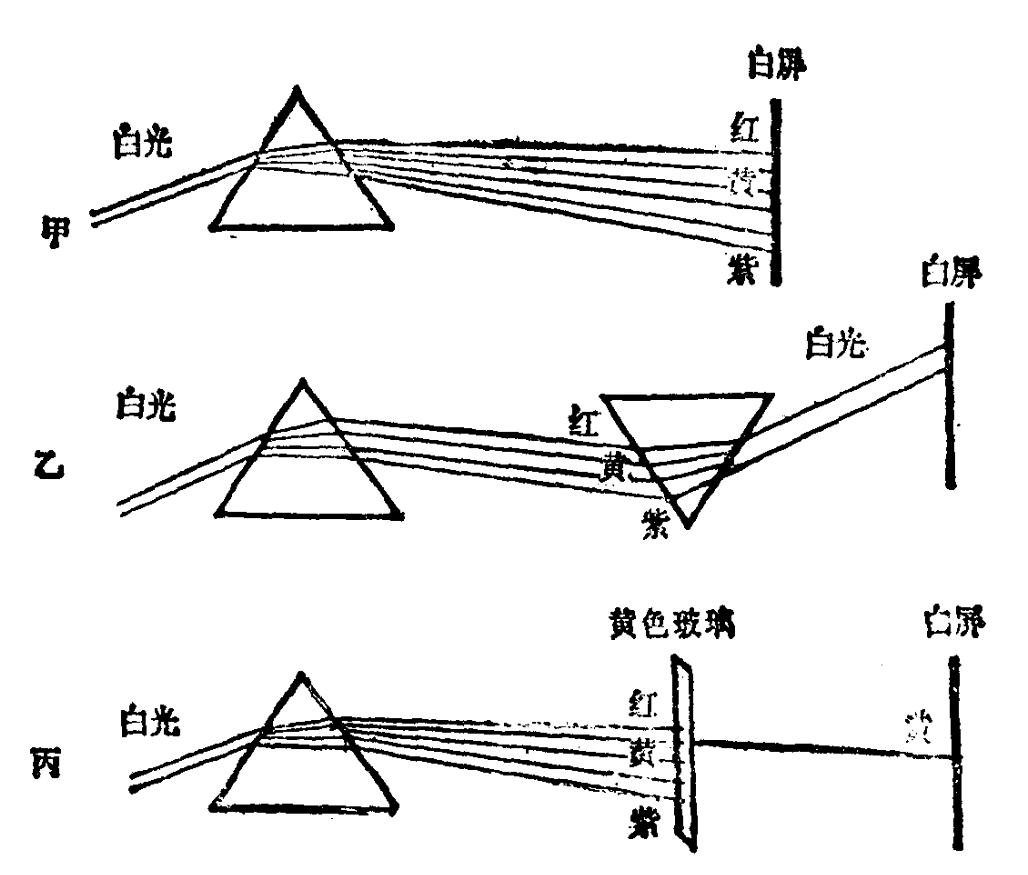
\includegraphics[width=0.7\textwidth]{../pic/czwl1-qy-1}
    \caption{}\label{fig:qy-1}
\end{figure}

专门研究物理学的人叫做物理学家。物理学家研究物理问题的方法是多种多样的,
但最根本的一条是进行观察和实验。伟大的物理学家伽利略从不忽略那
些看起来平常的细微现象,他仔细观察了从来没人注意过的大教堂里吊灯的晃动情况,
发现了悬挂着的物体在摆动中的等时性,从而在此基础上发明了简单方便的计时器——钟表。
在许多情况下,仅靠对自然现象的观察是不够的,还需要在人工控制的条件下对现象进行研究,
这就是做实验。例如,白光通过什么颜色的玻璃就成为什么颜色的光,那么是不是白光被色玻璃染了色,白光比色光更简单、更基本呢?
为了弄清这个问题,我们让一束白光射在三棱镜上,并在棱镜后面立一个白纸屏。可以看到,
透过棱镜射向屏的不再是白光,而分解成彩虹似的光带〈图 \ref{fig:qy-1} 甲)。
让这彩色光带再通过一个倒放的三棱镜( 图 \ref{fig:qy-1} 乙),色光又汇合成白光。
可见白光是由色光合成的,色光比白光更简单、更基本。
如果让彩色光带射到黄玻璃上( 图 \ref{fig:qy-1} 丙),透过的就只有黄光,其余色光都被吸收。
所以白光通过色玻璃不是被染了色,而是被吸收了一部分色光。
这个例子告诉我们,在物理研究中实验是多么重要。

在今后的学习中我们将不断看到,物理知识在生产技术中的应用是十分广泛的。
可以说,物理学的研究对生产技术的发展起了有力的促进作用。
反过来,人们由于要发展生产技术,也不断向物理学提出许多需要研究的问题,
生产技术发展了,又给物理学提供了越来越精良的仪器设备。
这样,生产技术的发展又大大地推动了物理学的研究。
现在,物理学的研究及其应用发展很快。
在物理学家中,既有许多人在不断探索新的物理知识,也有许多人跟工程技术人员合作,
努力把物理研究成果运用到国民经济的各个部门中去。

同学们就要开始学习物理知识了,为了学好物理知识,应该注意下面的几点建议。

第一,要重视观察和实验。物理中的规律性的知识都是从物理现象中抽象概括出来的,
因此,重视观察和实验,对学好物理知识有特别重要的意义。
在物理课上,教师将要演示各种物理现象,要仔细观察。
同学们还要亲自动手做一些实验,要弄懂它的道理,认真细致地操作。
此外,课本中还有一些小实验和实验题,要设法找一些简单的器材来自己做一做,试一试。
我们一定要懂得,只有通过细心观察物理现象,自己动手实验,才能真正掌握物理知识。

第二,要重视理解。对于物理知识,要力求理解它。所谓理解是指当提到某一物理知识的时候,
脑子里能够想到跟它有关的物理事实,知道它的应用,了解它跟有关知识的联系,而不是只记住结论。
另外,我们在理解物理知识的同时,还要力求理解物理学家是用什么方法,经过怎样的思考来探索这些知识的。
这样,我们就能够逐步懂得研究物理问题的方法,随着知识的增长,使自己的能力和才干也不断增长。

第三,要重视理论联系实际。我们在日常生活和生产劳动中,经常会遇到大量的物理现象,
遇到许多需要解决的物理问题。我们应该努力把所学知识用到实际中去,力求能解释一些现象,
解决一些简单的实际问题,课本中也有一些联系实际的练习题,对这些练习题,
要联系自己的实际经历多想想,不要只满足于得到一个解答。搞好理论联系实际,
不但可以使我们的知识学得更好更活,还可以培养我们分析问题和解决问题的能力。

同学们,我国各族人民,正在中国共产党的领导下,为把我国建设成农业、工业、
国防和科学技术现代化的社会主义强国而努力奋斗。我们一定要努力学好包括物理在内的科学文化知识,
以便将来成为有用的人材,在实现祖国的四个现代化中作出自己的贡献。

